
\documentclass[11pt,a4paper]{article}
\usepackage[utf8]{inputenc}
\usepackage{amsmath,amssymb}
\usepackage{graphicx}
\usepackage{hyperref}

\title{The Vacuum of Being\\\large A Philosophical and Scientific Inquiry Into the Substrate of Reality}
\author{Versão 2.0 (Jun/2025)}
\date{}

\begin{document}

\maketitle
\tableofcontents

\section*{Glossário}
\begin{description}
\item[Vácuo (𝒱)] estado fundamental de todos os campos.
\item[Substrato] 𝒱 interpretado como suporte ontológico de todas as modalidades.
\item[Modalidade] configuração estável (matéria), propagante (energia), oculta (matéria escura) ou homogênea (energia escura) de 𝒱.
\item[Estruturação $\Sigma$] métrica que quantifica a coerência topológica de 𝒱.
\end{description}

\section{Fundamentos e Definições}
Apresentamos o formalismo mínimo que viabiliza a hipótese...

\subsection{Lagrangiana efetiva}
\begin{equation}
\mathcal{L} = \sum_i \left[\frac12(\partial_\mu\Phi_i)^2 - V_i(\Phi_i)\right] + \lambda \Psi + \alpha\,\frac{\Psi^{2}}{M_\text{Pl}^{2}}.
\end{equation}

\section{Modalidades do Vácuo}
\begin{figure}[h]
\centering
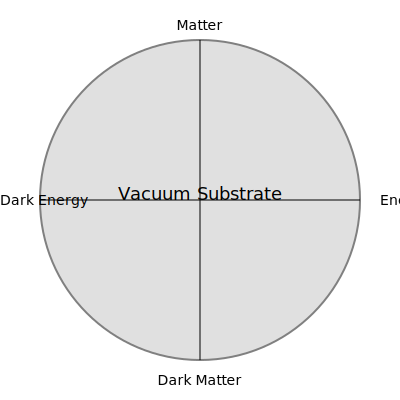
\includegraphics[width=0.6\textwidth]{mapa_modalidades.svg}
\caption{Mapa das quatro modalidades do vácuo.}
\end{figure}

\section{Previsões e Falsificabilidade}
Tabela resumida de previsões observacionais exclusivas...

\section{Objeções e Respostas}
Discussão crítica das principais objeções...

\section{Conclusão}
O vácuo é interpretado como universo em standby...

\end{document}
